\documentclass[fleqn,10pt]{wlscirep}
\usepackage[utf8]{inputenc}
\usepackage[T1]{fontenc}
\usepackage{bm}
\usepackage{siunitx}
\DeclareSIUnit{\Bit}{~Bit}


\title{Improving Pooling-Strategies for Increasing the Testcapacity and Reliability of RT-qPCR of Samples with low prevalence} %we should but SARS-CoV-2 somewhere...


%improve order of authors maybe use a circle (it's a really old list.)
\author[1,*]{Leo T. Peters}
\author[2]{Leonhard Kuboschek}
%\author[1,2]{Ruth}
\author[2]{Pranav Kumar Shadamarshan}
%\affil[1]{Affiliation, Department, City, Country}
%\affil[2]{Affiliation, Department, City, Country}

%\affil[*]{e-mail: leo.peters@tum.de}


\begin{abstract}

\end{abstract}
\begin{document}

\flushbottom
\maketitle

\thispagestyle{empty}

\section{Introduction}
Covid-19 has been taking over the world like a wildfire and the economies of
countries have succumbed to it. One of the main reasons being inefficient
testing strategies. Not only does a country need high testing capacity but also
faster testing capability. With faster and efficient testing strategy, a country
knows where it stands amidst this pandemic. For instance, South Korea in
the first week of its critical period had already conducted 300,000 tests,
establishing 600 test centres across the country. It had halved the number of
infections in just a week [1]. On the other end of the spectrum, Italy and US
has/is failing to cope up with the pandemic. So much so, Italy could not keep
up with the pandemic because they did not know where they stood in the
curve because of the inefficiency in testing samples. The delay in testing has
and is still costing lives [1-3]. The take home message from these scenarios is
that high capacity testing provides more information upon which a country
could take a standpoint and act in preparedness. So, we propose a strategy for
efficient testing of SARS-COV-2 by sample pooling.


\section{Methods}

\subsection{Information Theory}
A measure for the amount of information is the so called \glqq entropy\grqq{} and is associated with the unit \si{\Bit}. It forms the basis of information theory, which was initially developed by Shannon \cite{Shannon} and is mainly used in communication engineering. In this paper we will apply it to pool testing in order to estimate the potential of an optimal pooling strategy and to compare the developed strategies to such optimal performance. 

The relevance of information theory in the context of large scale testing can be understood as follows: The total amount of information on the patients state of a population is bounded, as we are looking at a finite number of people with a binary state (infected or not infected). By applying pool testing, the information obtained by a test can be increased, which allows us to require less tests in order to evaluate the peoples state.

The amount of information carried by a Bernoulli distributed (or binary) random variable can be closely related to the information carried by a diagnostical test, which also yields a binary result (positive or negative).

Information theory tells us, that the entropy of such random variable is maximized, if its both outcomes are equally distributed. In this case the amount of information is \SI{1}{\Bit}. This is also the maximum information obtained by a single diagnostic test that does not allow any errors in result.

In the case of single testing with ideal tests the amount of information obtained by one test is equal to the amount of information carried by one patients state. This is why we need exactly one test per person if we conduct single testing.

The entropy of the populations state depends on the prevalence and can be estimated by regarding each patient as a binary random variable with probability equalling to the prevalence $p_{inf}$:

\begin{equation}
H(p_{inf}) = -p_{inf} \cdot \log_2(p_{inf})-(1-p_{inf}) \cdot \log_2(p_{inf}) \si{\Bit}
\end{equation}

\begin{figure}[ht]
	\centering
	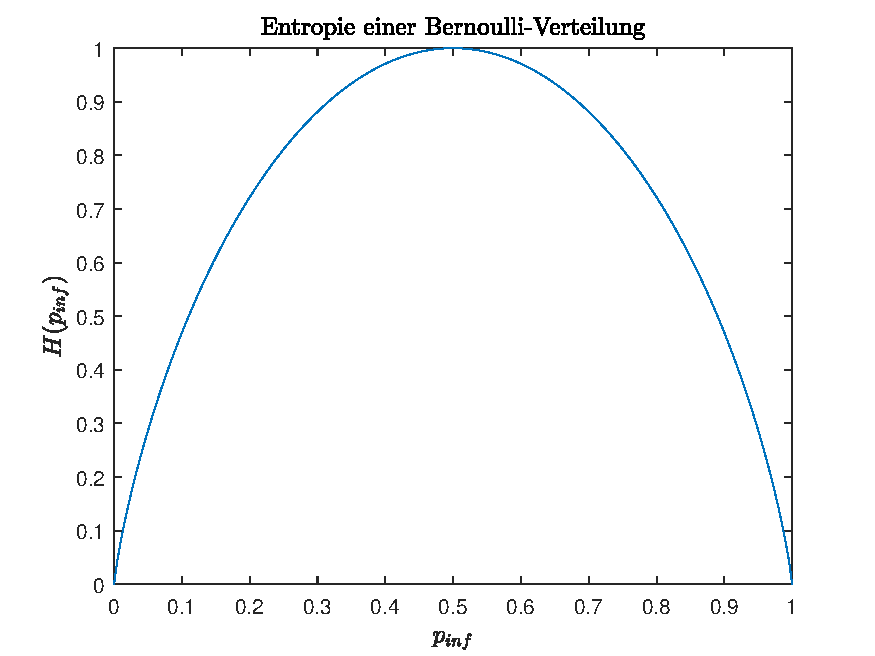
\includegraphics[]{pics/Bin_Entropie.pdf}
	\caption{Amount of Information obtained by a single and ideal test vs. prevalence $p_{inf}$}
	\label{fig:bin_entropie}
\end{figure}

Fig. \ref{fig:bin_entropie} shows a maximum in entropy of a test, if its outcome is equally distributed. It is interesting to note, that the entropy only varies slightly for small deviations from the optimum, while it drops to zero, when the prevalence is $0$. This means that single testing cannot be used efficiently at low prevalences. Prevalences above $0.5$ will not be regarded in this work.

By pooling samples together, we end up with a mix. We can increase the probability of such mix containing at least one positive sample. For low prevalences this leads to a higher amount of informtion obtained by one test conducted on this mix, when comparing it to single testing. This will be further carried out in section \ref{sec:analytics}.

Another important measure from information theory is mutual information. It indicates how much information of one random distribution can be obtained by another random distribution. If a diagnostic test was never leading to an error, the distribution of a persons state and of the test result a closely coupled, which results in the mutual information being equal to the entropy of the person's state. If however errors occur, the information lost during the conduction of a test (through false negatives and false positives) is the difference between the information of the person's state and the mutual information, which is depicted in fig. \ref{mutual information}. In the case of an imperfect diagnostic test, it can be useful to maximize the mutual information between the population's state and the test results instead of maximizing the entropy.

%insert picture of mutual information from wikipedia here.

Another use for the mutual information is the evaluation of conducting multiple diagnostic tests on subsets of a bigger pool of samples. Just as it is desirable to increase the mutual information between the population's state and the test results, it is also desirable to decrease the mutual information between the test results of multiple tests. This originates in the idea, that obtaining the same information by multiple tests will not increase the overall information retrieved.

The concept of mutual information will only be used as an instrument to emphasize differences between strategies, while it will not be used for optimization as part of this work.


\subsection{RT-qPCR}

\subsection{Assumptions}

\subsubsection{PCR simple}

\subsubsection{PCR dilution dependent}

\subsubsection{Viral Load}
The severity of the viral infection is characterized by its number of RNA copies in the patient sample. Clinical samples have shown around 1.6 x 106 RNA copies/ml [5]. The minimum amount required to analyse the sample is 400 RNA copies/ml [6]. This would technically mean that we could dilute a sample 4000 times and still be able to detect it. Pooling multiple samples would dilute the samples, but within a certain range would still be detectable. A test concluded that an interpretable signal was obtainable by pooling 31 samples together [7]. For a good strategy design, we would require as many trustable data we could get. The sensitivity and specificity, False Positive and negative rates of RT-qPCR, real time statistics of the infection in a country, and we hope to also design a strategy based on the symptoms. Currently 90% of the patients display symptoms of fever, 75% cough, 40 – 70% fatigue and 20 – 25% fluid secretion (sputum) [8].

%let us insert the distribution of viral load as a histogram or table here.

\subsection{Strategy Evaluation Measure}
- Sensitivity, specificity

- PPV, NPV

- Problems arising from bad values

\subsection{Modelling Strategies}
- Monte Carlo Simulation in MATLAB 

- Indiv Testing (no MC needed)

- State of the Art Pool Testing

Our aim for the strategies is to pool multiple sample together for better data obtainment. For this we have several pooling-approaches in mind.
The first one we called CoSplit. This approach is the only approach we simulated yet. Aim of CoSplit is to get the maximum information gain out of the first test and to split the pools up recursively, if the test turns out to be positive. For that we select the ideal start group size regarding the expected prevalence and pool all samples of this group together. If the result of the test is positive we split the group and test every subgroup. We do this until the group size is 1. In case of a negative test result we assume all samples of that pool are negative as well. Therefore there is no need to split negative tested groups into subgroups. Indeed in order to get a more precise result and reduce the number of false test results a retest of a negative tested group is being simulated as well. 
Yelin et al. describe the results of a COVID-19 RT-qPCR test in multi-sample pools. They came to the conclusion „that a single positive sample can be detected even in pools of up to 32 samples, with an estimated false negative rate of \SI{10}{\percent}“ (Yelin et al. 2020). 
As an example if we choose a start group size of 32 persons and a split factor of 2 we would mix up the samples of 32 persons and test this sample pool. If the result is negative we would assume (if an additional retest ist also negative) that all of the 32 persons are negative. In case of a positive result we would split the group and mix pools with 16 samples each and test these two pools again. A positive tested group would be split into 8-sample-pools and tested again. This goes on until the infected patient whose sample causes the positive pool test result is identified. In order to account for such detection limits when designing the strategy, we also decided to conduct simulation while limiting the maximum pool size.
% I would prefer not to use this argument here if at all. In the above mentioned paper of Yelin et al. each of the five positive samples were detected after 37 cycles even though they were diluted with 15 negative samples. Assuming that a pool of 16 samples has a lower false negative rate a start group size of 16 persons might be even better.

%I would prefer an outline on the square method.
%Sliced Cube
%Another approach we had in mind focuses not on the maximum information gain, but on receiving a faster result and on testing persons multiple times in order to decrease false results. Therefore we arrange the to-be-tested persons into multidimensional arrays.
%Again assuming that a good pool size is consisting of 16 samples we use 16-sample-pools for the following example. So if the people who should be tested are arranged in a 3-dimensional array/cube with an edge length of 4 and then slice this array/cube in every dimension into 4 slices each slice would contain 16 people. The whole array/cube would contain 64 (4^3) people.
%With this pooling method we would be able to reduce the number of tests from 64 test (if each person is tested with one test) to 12 tests (one test for each slice of the array/cube). Theoretically (if we assume the PCR test is always right and neglect the circumstance that the PCR-test could be false) this method has an unambiguous result if not more than one person of the group is infected. #1
%To increase the probability for getting an unambiguous result in cases of two or more infected people in the group and as an approach to cope with the possibility that a PCR-test is false (due to theoretically impossible results) more tests based on sample pooling could be added. One way of doing that is a diagonal slicing of the array/cube. For every dimension 8 more tests could be added (four slices for direction from upper left to lower right and four for upper right to lower left). Therefore 24 (4*2*3) additional tests would be needed. 


%#1 [insert calculation regarding prevalence and the expected number of infected in a group of 64 people]



\section{Analytical Optimization}
\label{sec:analytics}
- Group size Optimization for Standard pool test

- Group size Optimization for first CoSplit-Test with perfect PCR

Bei Durchseuchungsgraden kleiner $0,5$ bzw. \SI{50}{\percent} nimmt die Entropie zunächst langsam ab, konvergiert jedoch gerade am Ende schnell gegen Null. Das zeigt, dass ein Test bei einer Einzeltestung der Proben bei niedrigem Durchseuchungsgrad nicht effizient genutzt werden kann.
Durch eine Vermischung von Proben, erhalten wir eine neue Probe, deren Anzahl an positiver Teilproben binomialverteilt ist. Im folgenden wird ein solcher Probenmix als positiv bezeichnet, wenn sich darin mindestens eine positive Teilprobe befindet und sonst negativ. Jede Teilprobe ist stochastisch unabhängig mit der Wahrscheinlichkeit $p_{inf}$ positiv. Die Wahrscheinlichkeit für einen positiven Probenmix lautet nun
\begin{equation}
p_{n,inf}(p_{inf}) = 1-(1-p_{inf})^n 
\end{equation}
wobei $n$ die Anzahl der Teilproben im Probenmix entspricht. Ersichtlich ist, dass durch die Vermischung von Proben der Informationsgehalt eines Tests über den gesamten Mix erhöht werden kann. 

Anhand dieser Gegebenheit lässt sich für einen empirisch ermittelten Durchseuchungsgrad eine Optimale Gruppengröße bestimmen, deren   


\section{Simulation Results}

\subsection{Single Testing}

\subsection{State of the Art Pool Testing}

\subsection{CoSplit simple}

\subsection{CoSplit with Retesting}

\subsection{CoSplit with Poolsize Limit}



\section{Conclusion}

- Test capacity increasable. Test efficiency is around XXXX % depending on the redundancy
- Redundant testing shows improvement in Specificity
- Scaling of the number of retests with the prevalence leads to almost constant PPV.
- Pool Size limits decreases the efficiency at very low prevalences but increases the sensitivity.

\section{Further Research}
- more accurate data for PCR sensitivity (or even more detailed model)
	- use more sources
	- conduct own experiments
- more accurate data for viral load

- different strategies (e.g. matrix arrangement)

- optimize for best pandemic suppression
	- consider retesting after n days
	- compare pool testing and individual testing for different scenarios 
	
- extend model to other diagnostic tests


% \section*{Main text heading 1}

% Please use headings/subheadings to break up the text. Main headings should be no more than 38 characters, including spaces.

% \subsection*{Subheading 1}

% Subheadings should be no more than 39 characters, including spaces. In the final layout, subheadings will be in-line and thus followed by a full stop.

% \subsubsection*{Second-level subheading 1}
% Second-level subheadings should be no more than 70 characters, including spaces.

% \begin{figure}[ht]
% \centering
% %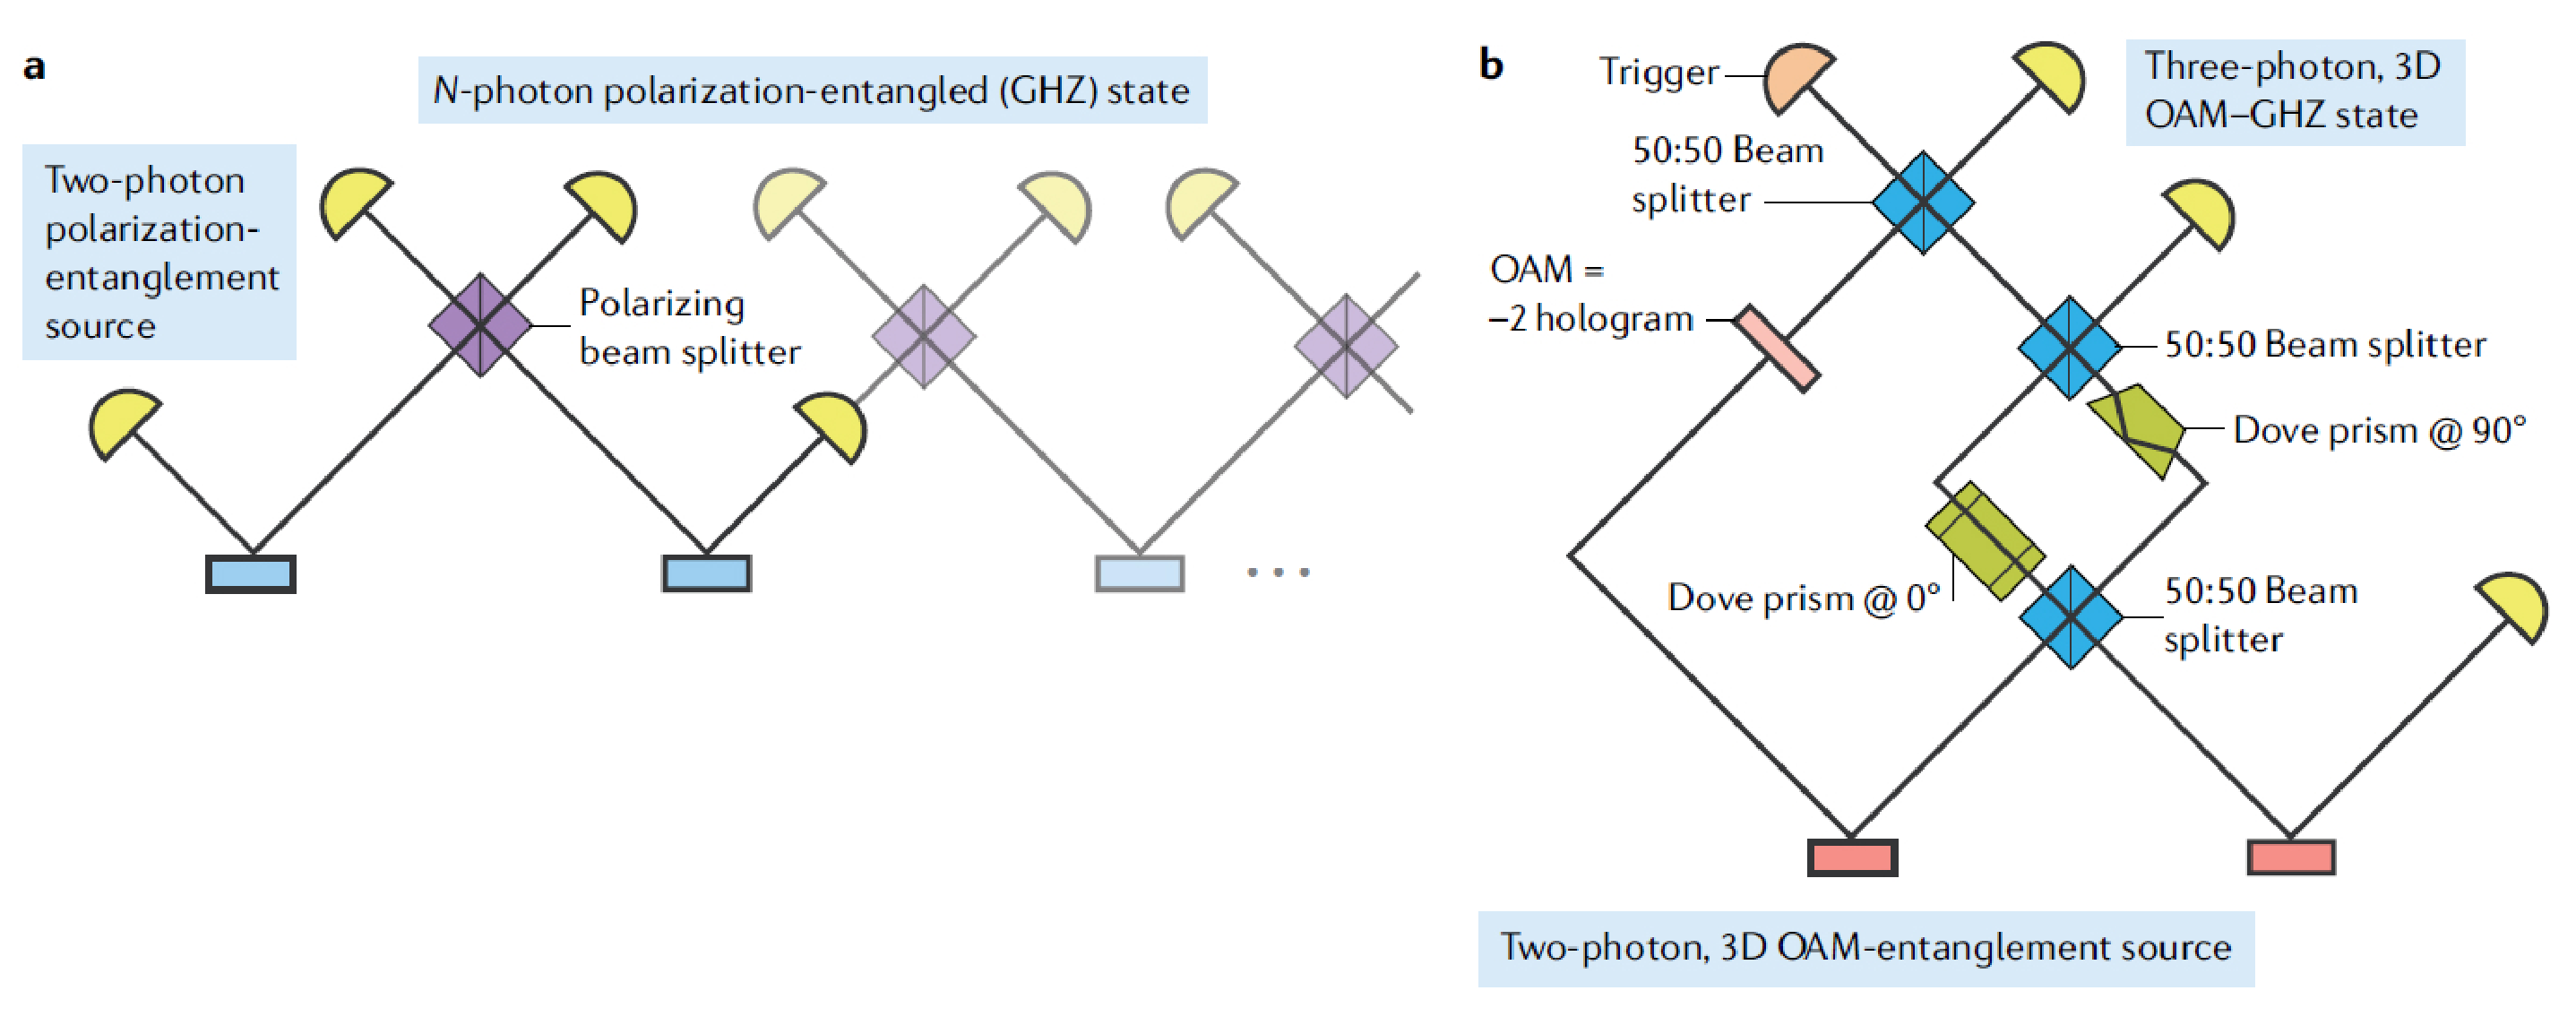
\includegraphics[width=\linewidth]{fig}
% \caption{\textbf{Title.} a | Text. b | Text. c | Text. d | Text maximum 250 words. Panel a is adapted/reproduced with permission from ref.123, Springer Nature Limited. Panel b is adapted/reproduced with permission from ref.124, Publisher Name.}
% \label{fig}
% \end{figure}



% \begin{table}[ht]
% \centering
% \begin{tabular}{|l|l|l|}
% \hline
% Particle & Mass & Charge \\
% \hline
 % \multicolumn{3}{|c|}{Charged particles}\\
% \hline
% Electron & $9.10938356(11)\times10^{-31}$ kg & $-1e$ \\
% \hline
% Proton & $1.672621898(21)\times10^{-27}$ kg & $+1e$ \\
% \hline
 % \multicolumn{3}{|c|}{Neutral particles}\\
% \hline
% Neutron & $1.674927471(21)\times10^{-27}$ kg & $0$ \\
% \hline
% \end{tabular}
% \caption{\label{tab}Tables have titles but no captions are allowed. All symbols and acronyms used in a table should be defined in a footnote. Example: Here $e$ is the elementary charge.}
% \end{table}


% \noindent\textbf{Acknowledgements}\\
% E.g. Funding agencies.\\

% \noindent\textbf{Author contributions}\\
% Please describe the contributions made by each author.  Please use the initials of the individual author to explain these contributions.  These contributions are also required when you upload the files to our submission website.\\

% \noindent\textbf{Competing interests}\\
% Nature Journals require authors to declare any competing interests in relation to the work described. Information on this policy is available \href{http://www.nature.com/authors/policies/competing.html}{here}. \\



% \noindent\textbf{Supplementary information (optional)}
% If your article requires supplementary information, please include these files for peer-review. Please note that supplementary information will not be edited.


\end{document}